\documentclass{article}
\usepackage[margin=1in]{geometry}
\usepackage{graphicx}
\usepackage{xcolor}
\usepackage{float}
\usepackage{amsmath}
\usepackage{cite}
\usepackage{hyperref}
\usepackage{indentfirst}
\graphicspath{{..} {./images}}

\definecolor{navy-blue}{rgb}{0.22,0.38,0.71}

\renewcommand{\contentsname}{\vspace*{-2\baselineskip}}

\hypersetup{
	colorlinks,
	linkcolor=black,
	urlcolor=blue,
	citecolor=black
}
  		
\begin{document}
\begin{titlepage}
	\centering
	{\huge Lab 8 - SDR: Software Defined Radar}\\[0.25 in]
	
\includegraphics[width=0.6\textwidth]{ua_logo.png}\\[0.25 in]
	{\large \textbf{ECE 531 - Software Defined Radio\\[0.25 in]
	April 28, 2025\\[0.25 in]}}
	{\large Owen Sowatzke, osowatzke@arizona.edu\\[0.05 in]
	Department of Electrical \& Computer Engineering\\[0.05 in]
	University of Arizona, Tucson, AZ 85721\\[0.5 in]}
	\hypersetup{linkcolor=navy-blue}
	\noindent\hrulefill
	\tableofcontents
	\noindent\hrulefill
\end{titlepage}

% \setlength{\parindent}{0pt}

\section{Introduction}
%Introduction to the laboratory experiment, including a brief description of the objectives and goals.

In this lab, we create a monostatic continuous wave (CW) radar using our PlutoSDR. Our CW radar uses doppler beat frequencies to measure velocity, but it does not measure measure range. In our experiments, we specifically use our CW radar to measure the angular velocity of box fan blades. Then, we explain how we can improve our radar. The work that follows is divided into two sections. First, we provide the procedure for each of our experiments. Then, we discuss the results. 

\section{Procedure}
% Detailed explanation of the laboratory experiment, including the design, implementation, and testing of the system.

In this section, we provide the procedures for each of our experiments. We specifically use GNU radio to implement our CW radar. A block diagram for a sample CW radar implementation is attached in Figure \ref{fig::gnu_radio_block_diagram}.

\begin{figure}[H]
    	\centering
    \fbox{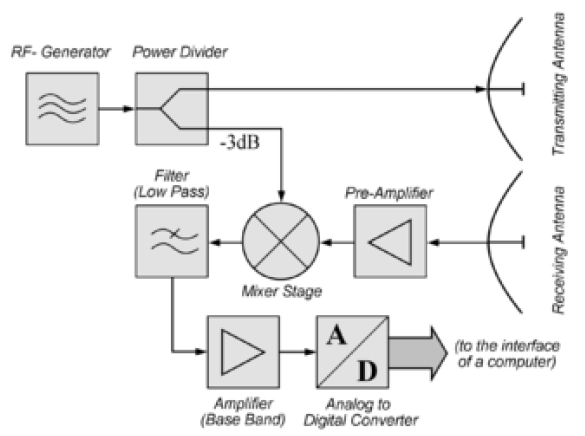
\includegraphics[width=0.5\linewidth]{cw_radar_block_diagram.png}}
    	\caption{RF Block Diagram for a Simple CW Radar \cite{charvat_2011_build}}
    	\label{fig::cw_radar_block_diagram}
\end{figure}

\noindent CW radars, such as the one shown, use the difference between the transmitted and received frequencies to measure the doppler shift of the target.

\begin{equation*}
	f_d = f_r - f_t
\end{equation*}

\noindent For a target with a velocity $v$, the doppler shift can also be approximated as follows:

\begin{equation*}
	\label{eq::dopp_shift}
	f_d \approx \pm\frac{2v}{\lambda}
\end{equation*}

\noindent Here the positive sign corresponds to a closing target and the negative sign corresponds to an opening target. Using the above equation and our measured doppler shifts, we can estimate the target velocity as follows:

\begin{equation*}
	v \approx \pm\frac{f_d\lambda}{2}
\end{equation*}

\noindent In this lab, we use our CW radar to measure the angular velocity of a box fan. Next, we explain the strong DC return in our waterfall plots and discuss physical changes that can be made to reduce the power of this return. Then, we discuss how an interfering signal could affect the operation of our radar and propose changes to make the design more resilient to interference. Finally, we discuss how the design can be updated to support range measurements.

\section{Results}
% Results and discussion of the laboratory experiment, including captured outputs, observations, and responses to laboratory questions.

In this section, we provide the results for each of our experiments. We specifically create a GNU radio flowchart, which implements a CW radio in our PlutoSDR. Next, we use our design to measure the angular velocity of moving box fan blades. Then, we discuss the short-comings of our design: DC return, no resilience to interference, and no range information. Finally, we discuss how we can improve our design to handle these short-comings. Our GNU radio flowchart is shown in Figure \ref{fig::gnu_radio_block_diagram}. 

\begin{figure}[H]
    	\centering
    \fbox{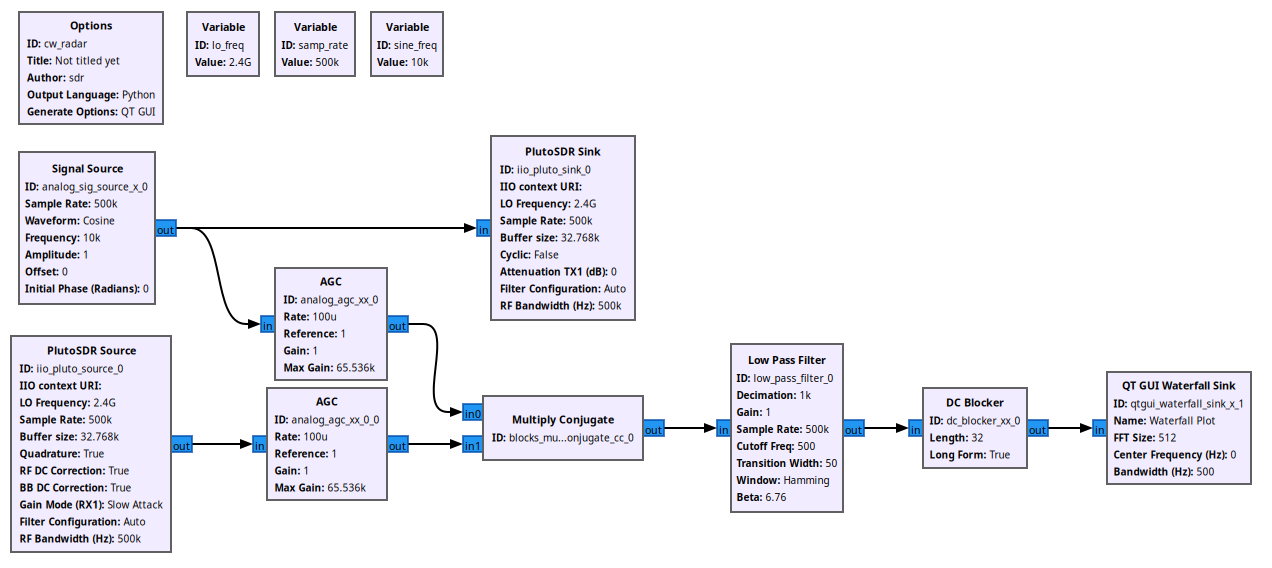
\includegraphics[width=0.7\linewidth]{gnu_radio_block_diagram.png}}
    	\caption{GNU Radio Flowchart which Implements a CW Radar}
    	\label{fig::gnu_radio_block_diagram}
\end{figure}

\noindent In this flowchart, we transmit a 10 kHz sinusoid centered about a 2.4 GHz carrier frequency. Then, we receive the sinusoid with a 500 kHz RF bandwidth and 500 kHz sampling rate. Note that our sampling rate is much greater than twice the highest frequency in our received signal (10 kHz plus a doppler shift), so we could further reduce our sampling rate if desired. However, if we do so, we should also reduce the RF bandwidth to reduce the amount of noise that aliases back into our spectrum. Next, we perform AGC on the received signal and signal source to maintain signal power. However, both these blocks can likely be removed from our design because our transmitted signal has a fixed signal power and because we are performing AGC in the PlutoSDR. Next, we multiply the received signal by the conjugate of the transmitted signal. This is equivalent to mixing our return down to DC. After we mix down, we should be left with a tone at DC (from clutter and leakage) and a tone at the doppler shift. The doppler shift of our returns will be small with respect to our bandwidth. As such, we apply a low-pass filter to our signal and decimate to a sampling rate of 500 Hz. At this sampling rate,we can unambiguously resolve doppler shifts up to $\pm 250\ \text{Hz}$ and radial velocities up to $\pm 15.625 \text{m}/\text{s}$. We also add a DC blocker before the waterfall plot to remove the clutter and leakage returns, which are much stronger than our target return.

%\begin{equation*}
%	f_d = \frac{2v}{\lambda}
%\end{equation*}

% \noindent We specifically choose  shift of 

Next, to measure the angle velocity of our box fan blades, we place our PlutoSDR in front of the fan and execute our flowchart. The waterfall plot that is generated during this experiment is displayed Figure \ref{fig::dopp_spectrum}. Note that our flowchart shows the doppler shift for three different fan speeds: slow, medium, and fast.

\begin{figure}[H]
    	\centering
    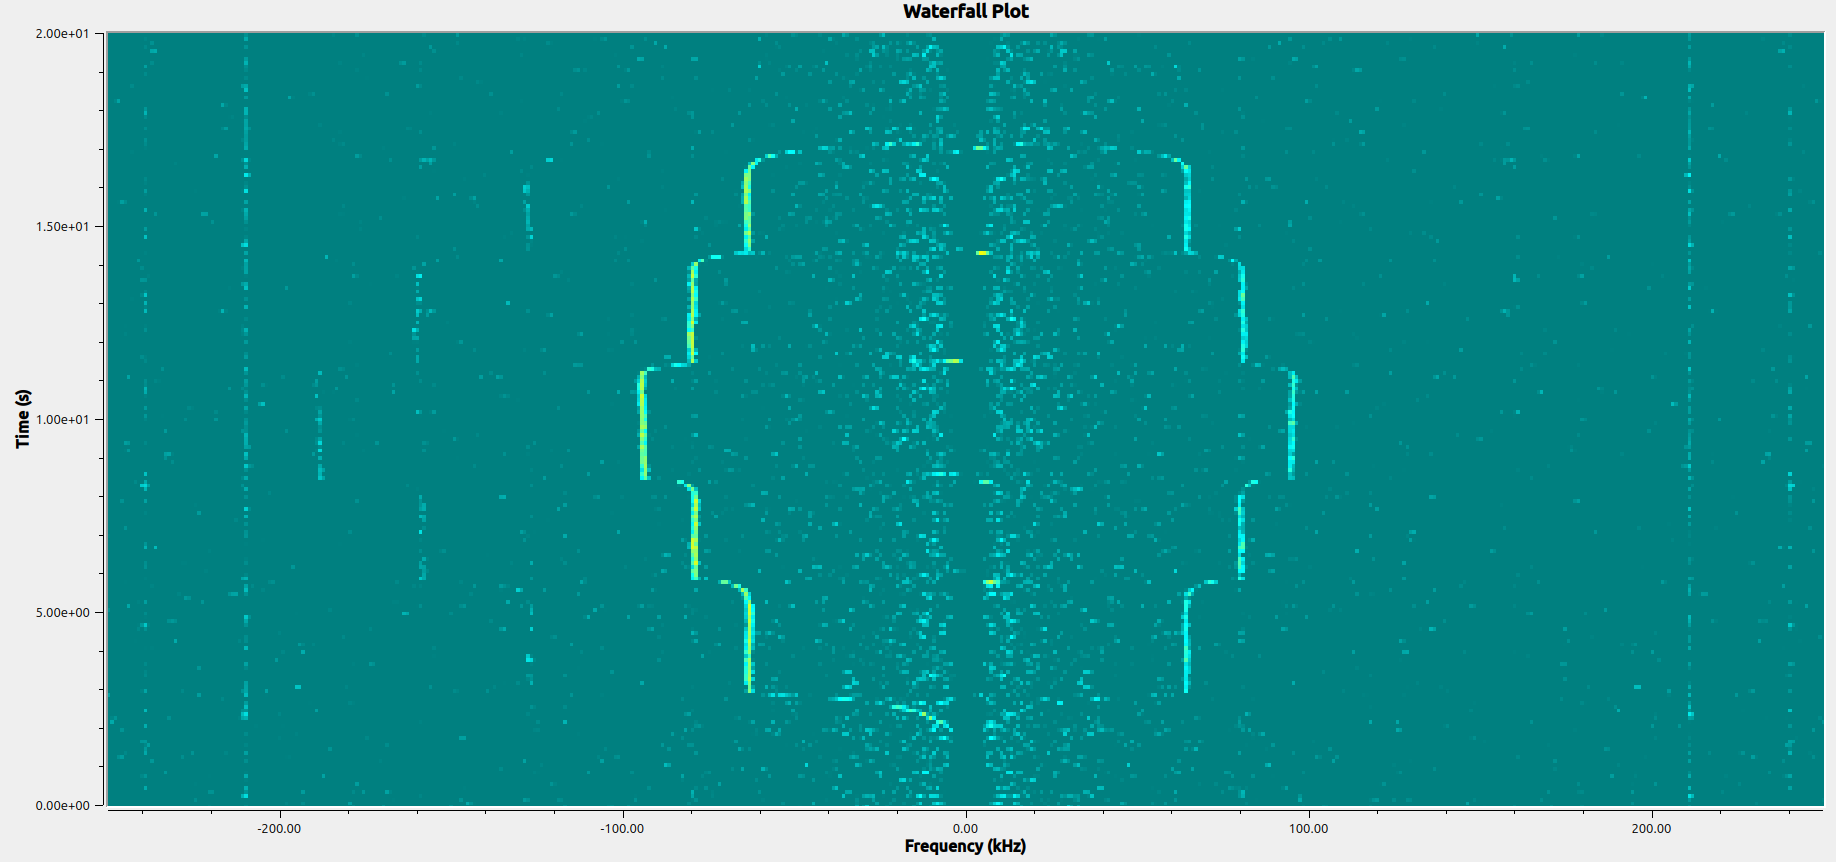
\includegraphics[width=0.9\linewidth]{dopp_spectrum2.png}
    	\caption{Waterfall Plot Displaying Doppler Shift from Box Fan}
    	\label{fig::dopp_spectrum}
\end{figure}

\noindent Using the waterfall plot, we measure doppler shifts of 63 Hz at low speed, 79 Hz at medimum speed, and 95 Hz at high speed. This corresponds to radial velocities of 3.9375 m/s, 4.9375 m/s, and 5.9375 m/s respectively. However, we have to be careful when mapping our radial velocity measurements back to angular velocities. To help with this mapping, we consider the setup shown in Figure \ref{fig::angular_velocity_measurement}. 
\begin{figure}[H]
    	\centering
    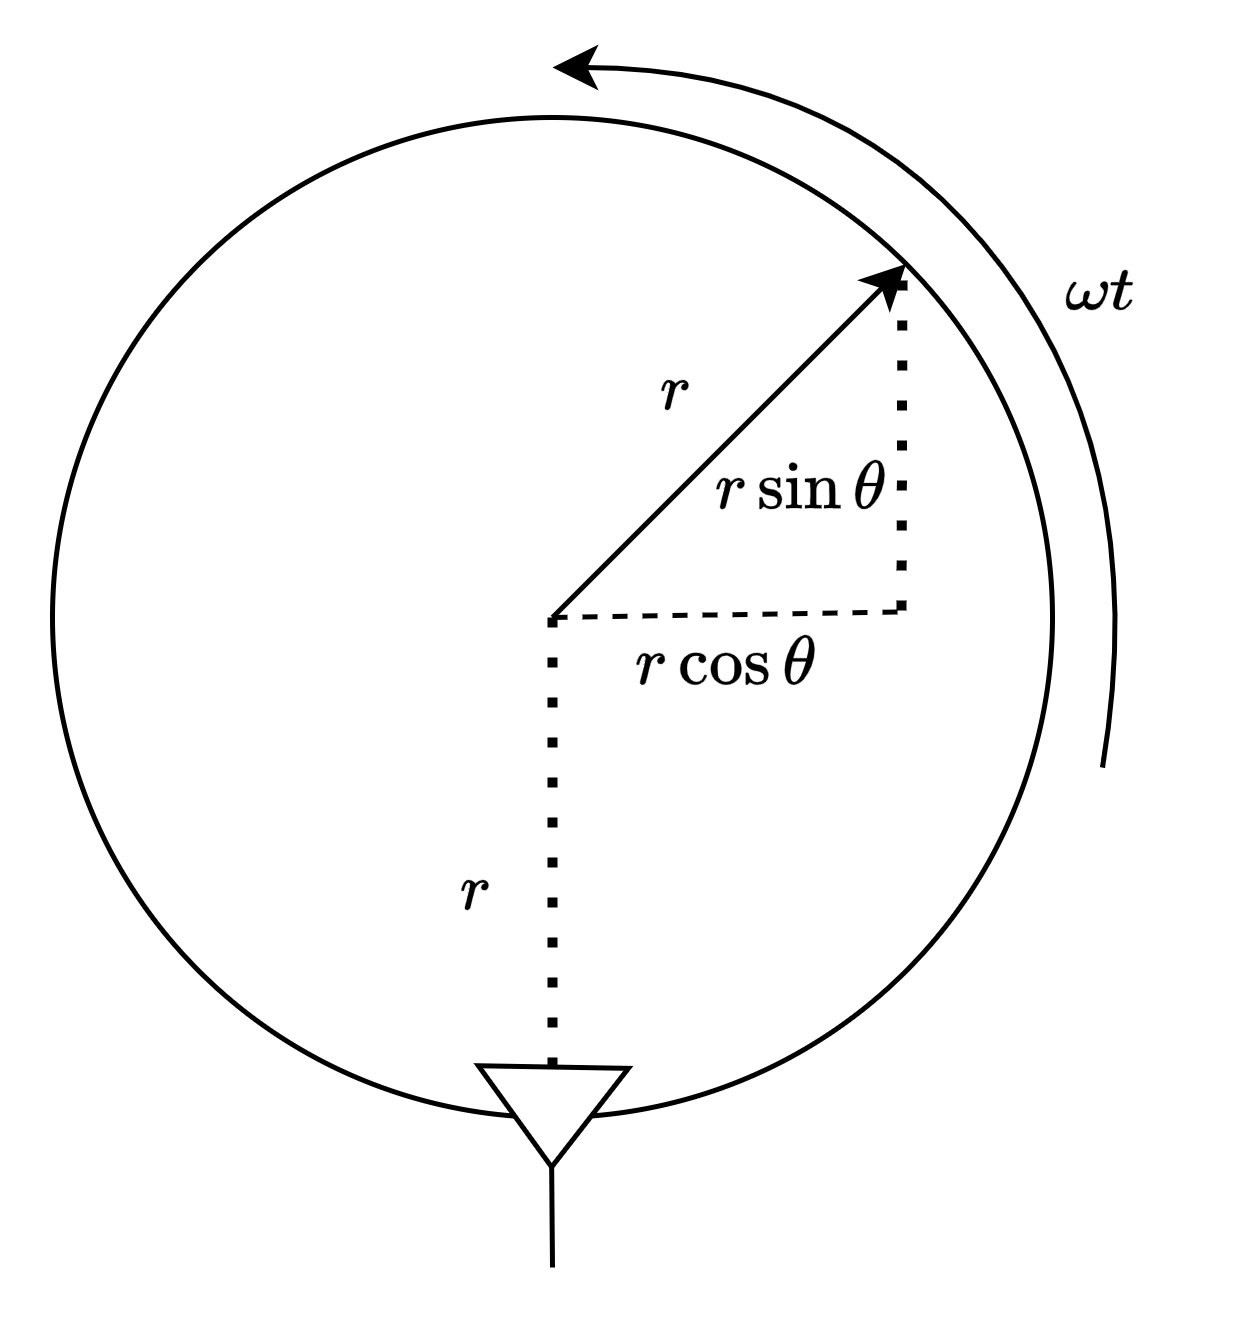
\includegraphics[width=0.4\linewidth]{angular_velocity_measurement.png}
    	\caption{Measuring the Doppler Shift of a Rotating Point Target}
    	\label{fig::angular_velocity_measurement}
\end{figure}

\noindent In this setup, we consider a point target which rotates around a circle of radius $r$ with an angular velocity $\omega$. We specifically measure the doppler shifts of our return when our antenna is placed at the base of the circle. Note that our antenna also extends some distance $d$ out of the page. This model is an oversimplification of our lab setup. However, it is still useful for our understanding. To solve for the doppler shifts, we first compute the radial distance between the target and point antenna. The resulting radial distance, $x$, can be computed for each angular position as follows:

\begin{equation*}
	x = \sqrt{r^2\cos({\omega}t)^2 + (r\sin({\omega}t) + r)^2 + d^2}
\end{equation*}

\noindent To obtain the radial velocity, we use MATLAB to differentiate the radial distance with respect to time. Then, we plug our results into Equation \ref{eq::dopp_shift} to compute the corresponding doppler shift. For this analysis, we choose representative values for the blade length and antenna position: $r = 0.25\ \text{m}$ and $d = 0.4\ \text{m}$. We also choose $\omega = 40\pi\ \text{rad}/\text{s}$ as a placeholder for our angular velocity. The doppler shift that results from our sample values is included in Figure \ref{fig::dopp_shift_vs_time}.

\begin{figure}[H]
    	\centering
    \fbox{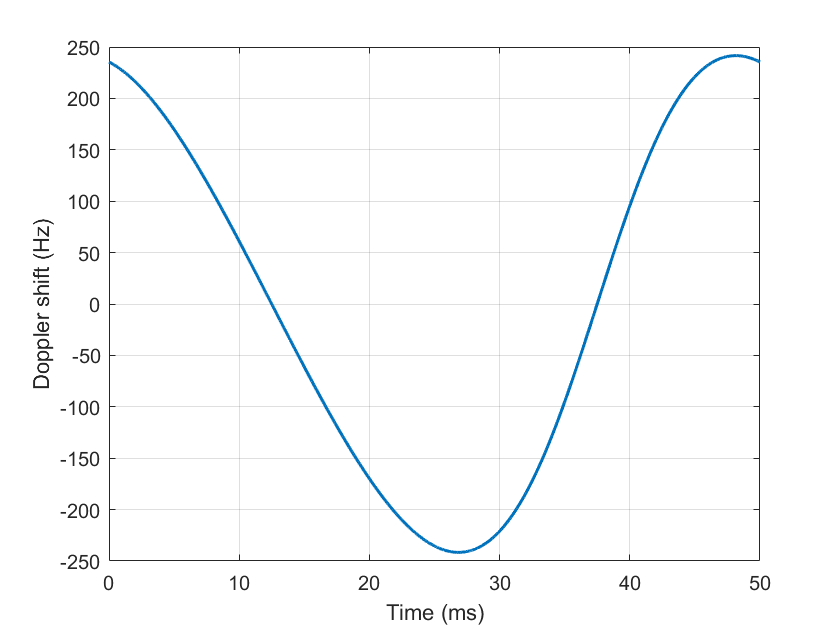
\includegraphics[width=0.5\linewidth]{dopp_shift_vs_time.png}}
    	\caption{Doppler Shift of Rotating Point Target Against Time}
    	\label{fig::dopp_shift_vs_time}
\end{figure}
 
\noindent We can understand this plot by referring to the test setup shown in Figure \ref{fig::angular_velocity_measurement}. Doing so, we find that the frequency decreases as we rotate away from the antenna and increases as we rotate towards the antenna. This time-varying doppler shift is known as the micro-doppler effect. It is also presented in the MATLAB documentation, which estimates the doppler shifts from a spinning helicopter blades \cite{matlab_micro_doppler}.

\begin{figure}[H]
    	\centering
    \fbox{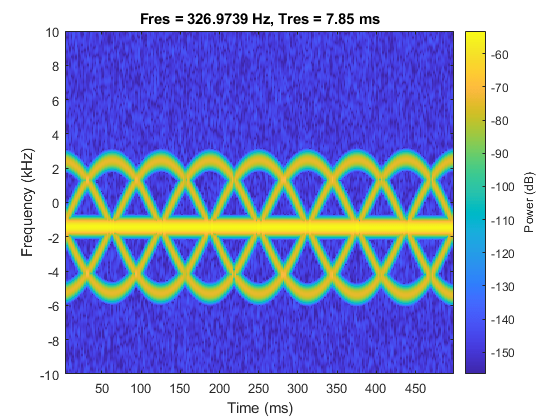
\includegraphics[width=0.5\linewidth]{micro_doppler.png}}
    	\caption{Doppler Shift Induced By a Spinning Helicopter Blades \cite{matlab_micro_doppler}}
    	\label{fig::micro_doppler}
\end{figure}

Depending on the duration of our FFTs, we may or may not see changing doppler shifts in our time-frequency plots. For the rotating point target we simulated, we captured data for a full rotation of the blades before taking the FFT. This results in a fixed-width spectrum which is shown in Figure \ref{fig::freq_response}.

\begin{figure}[H]
    	\centering
    \fbox{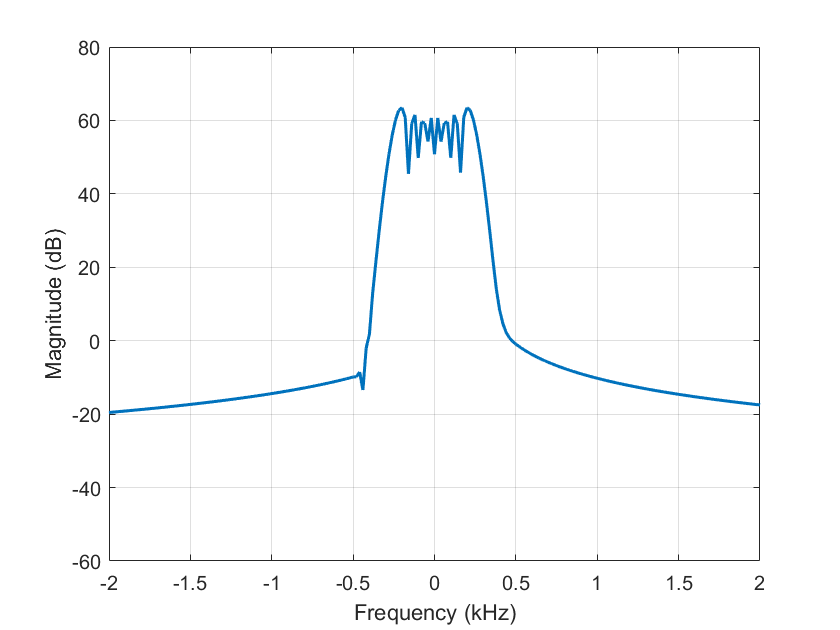
\includegraphics[width=0.5\linewidth]{freq_response.png}}
    	\caption{FFT of Rotating Signal Reflection}
    	\label{fig::freq_response}
\end{figure}

\noindent Note that the simulated spectrum is very different from our hardware results, which are included in Figure \ref{fig::dopp_spectrum}. How can we explain the discrepancies in our results? Our simulation results were collected over one period of the sinusoid, while each point in our waterfall plot was likely collected over multiple periods of the input signal. If we perform our FFT in simulation over multiple cycles of the input signal, we get the plot shown in Figure \ref{fig::freq_response_multi_cycle}.

\begin{figure}[H]
    	\centering
    \fbox{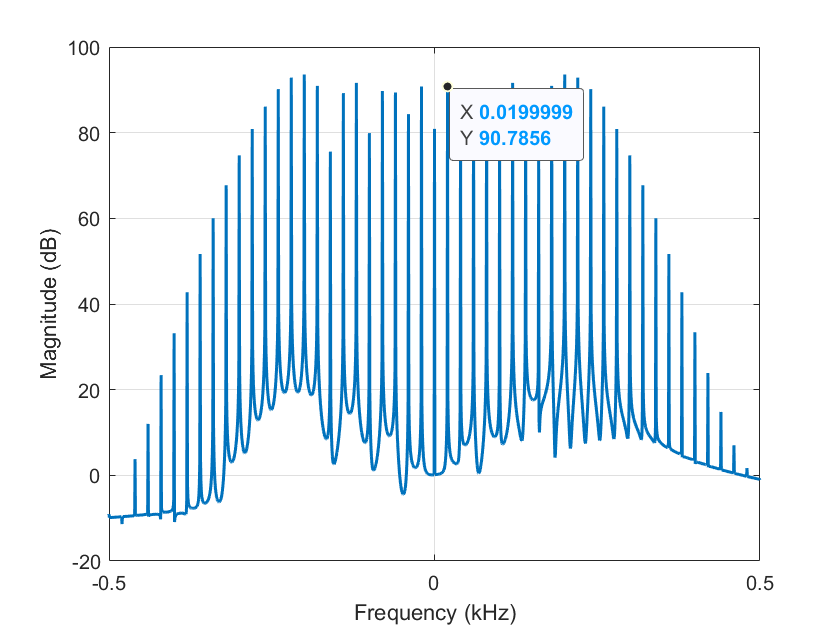
\includegraphics[width=0.5\linewidth]{freq_response_multi_cycle.png}}
    	\caption{FFT of Rotating Signal Reflection Over Multiple Cycles of Rotation}
    	\label{fig::freq_response_multi_cycle}
\end{figure}

\noindent Note that repeating our signal in the time domain has inserted zeros between the samples in our frequency response. This is analogous to how upsampling (inserting zeros between samples) leads to replication in the frequency domain. The frequency of our first harmonic (20 Hz) also corresponds to the configured frequency of rotation. We do see evidence of faint harmonics in Figure \ref{fig::dopp_spectrum}, which can be explained by this theory. We can better visualize these artifacts if we place the PlutoSDR closer to the fan, to boost the SNR. The results of this analysis are included in Figure \ref{fig::dopp_harmonics}.

\begin{figure}[H]
    	\centering
    \fbox{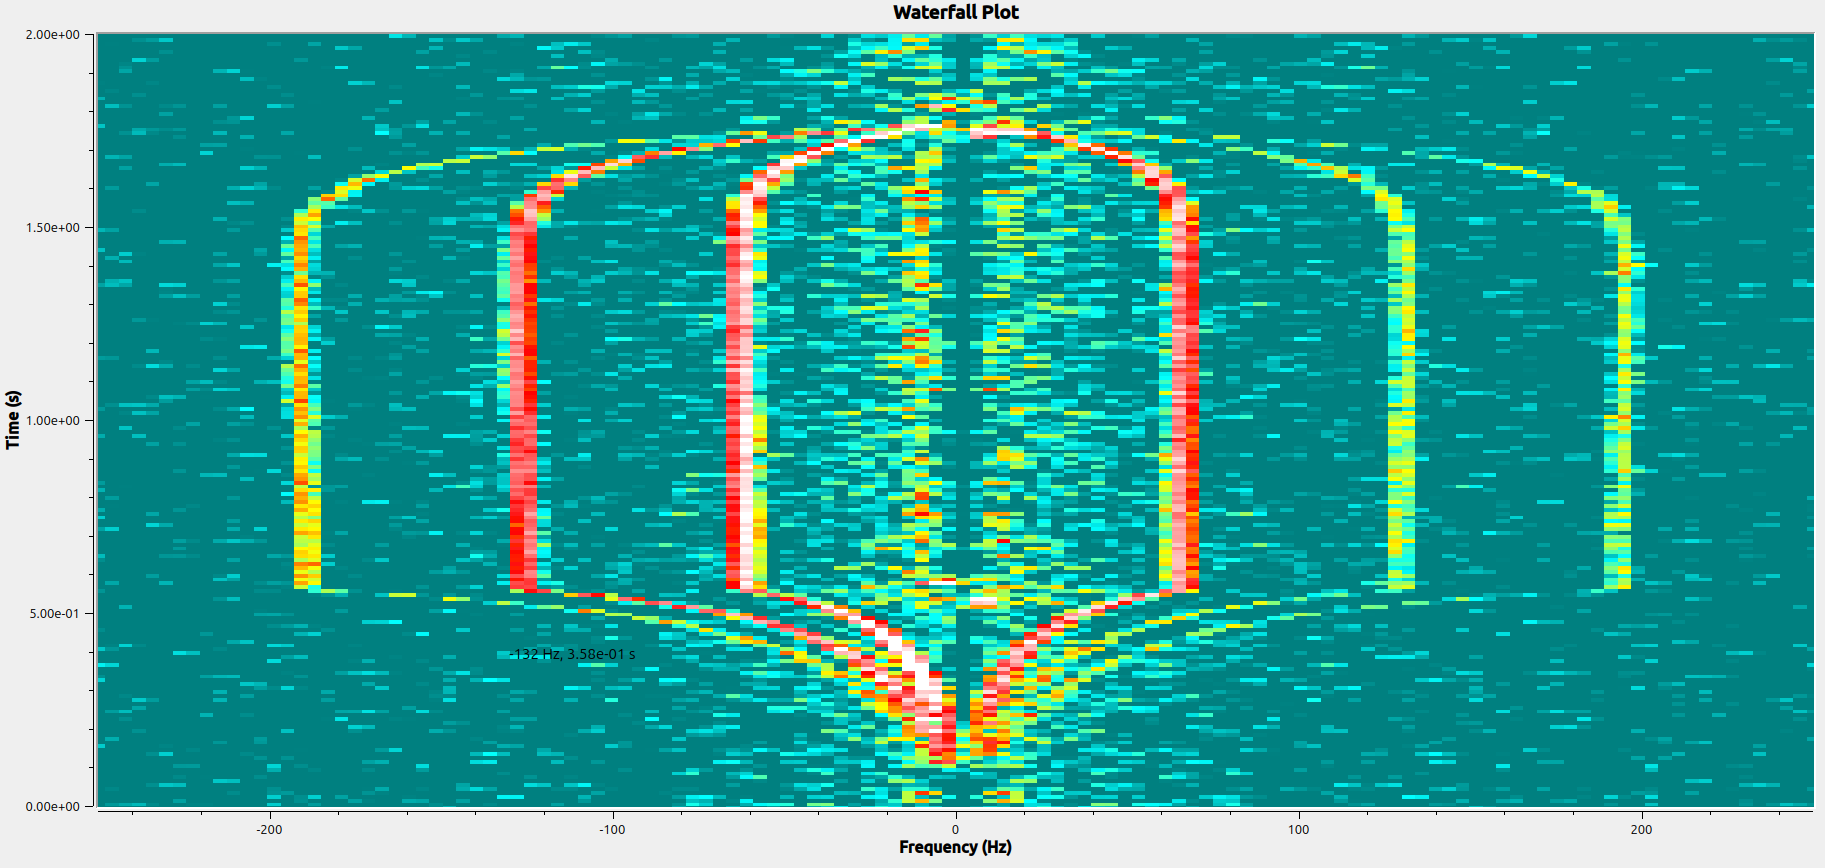
\includegraphics[width=0.75\linewidth]{dopp_harmonics.png}}
    	\caption{Data Captured with Pluto SDR Confirming Harmonics}
    	\label{fig::dopp_harmonics}
\end{figure}

\noindent In our Figure, we capture the fan being turned on at the lowest speed setting and then being turned off again. As soon as the fan is turned on, we see evenly spacing harmonics confirming the results shown in Figure \ref{fig::freq_response_multi_cycle}. We also monitored the sampled signal power at the output of the ADC with a QT Time Sink and did not see any clipping artifacts.

From our simulation results, we know that the frequency of the first harmonic is related to period of the signal. Therefore, we can use its frequency to compute the angular velocity. In our analysis, we also need to account for the number of fan blades because they will decrease the period of the signal and increase the resulting frequency. Our fan specifically had 5 blades. Therefore, we conclude that the angular velocities for slow, medium, and fast speeds are 63/5 rps, 79/5 rps, and 95/5 rps. These measurements correspond to 756 rpm, 948 rpm, and 1140 rpm, which are reasonable angular velocities for box fan blades.

Next, we consider some of the non-idealities present in our data. Two common causes of the DC return are clutter (from stationary returns) and transmitter leakage. We can minimize clutter with a tighter antenna pattern or by operating in an controlled environment, such as an anechoic chamber. However, it is usually not possible for us to constrain our environment. We can also achieve better antenna isolation by using a tighter antenna pattern. To reduce leakage, we can also consider other designs such as a pulsed doppler radar, which blank the receiver during transmission. However, pulsed-doppler radars may not be suitable for all applications (such as dealing with close range targets). However, for the purposes of the lab, we simply used a notch filter to remove the DC component of our signal.

We also consider the effect of interference, which would negatively impact our CW radar's operation. If the interference was from a wideband signal (such as 802.11 WiFi), it could cover the entire bandwidth of our signal and make detection more difficult. Conversely, if the interfering signal was narrow bandwidth (such as a tone), it could lead to false detections. To mitigate interference, we can do a few things. First, we should try to minimize the utilized bandwidth. In the sample flowchart, provided with the lab, the RF bandwidth was larger than the sample rate. A tighter RF bandwidth can prevent interference from aliasing back into our bandwidth. Additionally, if the interference is high power, a tight RF bandwidth can prevent the AGC from acting on interference and increase the number of bits used to represent our return. We can also implement more sophisticated techniques to handle interference. For example, we can use a coded waveform such as a Barker code or Zadoff-chu waveform to increase the coherent gain on our returns. Additionally, having a tighter antenna pattern can reduce the interference power and increase the power of our returns. If we had a ULA, we could even implement beamforming to null interference signals from different directions of arrival.

Another limitation of our design is that it cannot measure range. We can extend our design to measure range if we replace our sinusoid with a chirp. This is done in FMCW radars, for example, which we illustrate in Figure \ref{fig::fmcw_radar}.

\begin{figure}[H]
    	\centering
    	\fbox{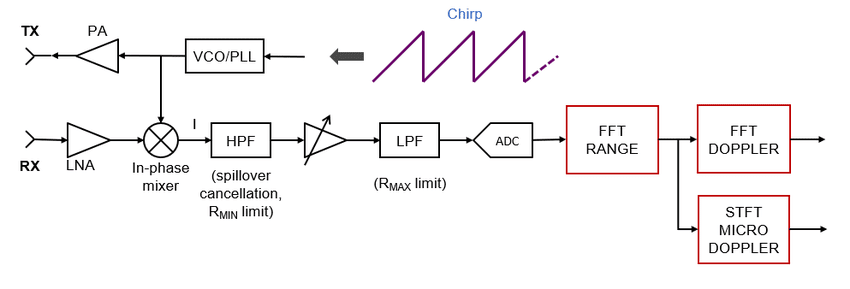
\includegraphics[width=0.6\linewidth]{FMCW Blockdiagram}}
    	\caption{Typical FMCW Block Diagram \cite{9613183}}
    	\label{fig::fmcw_radar}
\end{figure}
	
\noindent In an FMCW radar, we generate our chirp waveform with a VCO. The resulting transmit and receive signals are shown in Figure \ref{fig::fmcw_spectrogram}.

\begin{figure}[H]
    	\centering
    	\fbox{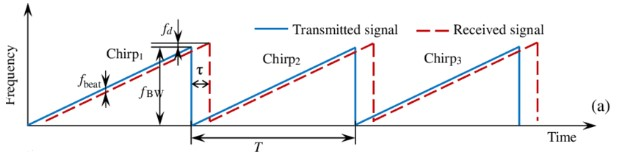
\includegraphics[width=0.6\linewidth]{FMCW Freq-Time graph}}
    	\caption{Time Frequency Plot for Transmit and Receive Signals.\cite{Long2019AssistingTV}}
    	\label{fig::fmcw_spectrogram}
\end{figure}

\noindent After mixing the receive signals with the transmitted signal, we get a tone with a frequency that is proportional to range. If we limit the maximum resolvable range, we can use a sample rate that is much lower than the chirp bandwidth. This significantly reduces the hardware cost. Then, we can use an FFT to measure the range as illustrated in Figure \ref{fig::fmcw_radar}. Additionally, we can measure doppler shifts by taking a slow-time FFT across pulses.

\section{Conclusion}
% Conclusions to the overall lab that discuss meaningful lessons learned and other takeaways from the assignment. (Important)

In this lab, we created a CW radar in GNU radio, which used our PlutoSDR to measure doppler shifts. These doppler shifts were proportional to the radial velocity of the targets. Using our flowchart, we specifically measured the angular velocity of fan blades in a running box fan. The running box fan generated a wide swath of doppler shifts. When the blades rotated closer to the antenna, we received positive doppler shifts. Similarly, when the blades rotated away from the antenna, we received negative doppler shifts. However, our waterfall plots did not show this wide swath of doppler frequencies. Instead, we observed harmonics because we captured multiple periods of our signal return. The frequency of the first harmonic was related to the period of the signal, which was in turn related to the angular velocity of the fan blades. Therefore, we were able to use the frequency of the first harmonic to solve for the angular velocity.

We also observed some non-idealities in our data. These included a strong DC return, sensitivity to interference, and no range measurement. The DC return in our data was a result of clutter and transmitter leakage. In the lab, we ignored the DC returns with a DC blocker. However, we learned that we could also minimize these returns using a tighter antenna pattern, a more controlled environment, and with alternative designs such as a pulsed doppler radar. Next, we found that interference could lead to reduced probabilities of detections and increased false alarm rates depending on the bandwidth of the signal. We learned that we could mitigate interference by reducing our RF bandwidth, using coded waveforms, using a tighter antenna pattern, or using beamforming (with a ULA). Finally, we discussed how we could measure range using an FMCW radar. The FMCW radar transmits a chirp waverform and mixes the received signal with the transmitted signal. After filtering, this results in a beat frequency with a frequency that is proportional to range. We can measure the frequency of this tone (and the resulting range) with an FFT. Additionally, we can maintain our ability to measure doppler shifts by taking a slow-time FFT across pulses.
 

  %were able  how to measure the radial velocity of our target.

% doppler shifts we measured were proportional to radial velocity, and were were   We specifically  with our PlutoSDR. For our implementation, we 

\bibliographystyle{IEEEtran}
\bibliography{sources}{}

\end{document}